% !TeX encoding = UTF-8
%
\documentclass[
%
	fontsize = 12.1pt,
	paper    = A4,
	pagesize = auto
%
]{scrreprt}



% !TeX encoding = UTF-8
%
% LaTeX-Pakete.
%


%
% Neue Deutsche Rechtschreibung.
%
\usepackage[ngerman]{babel}

%
% Automatische Kodierung vieler Sonderzeichen.
%
\usepackage[utf8x]{inputenc}

%
% Z.B. Symbol: Schwarzer Stern.
%
\usepackage{amssymb}

%
%
%
%\usepackage{tikz}

%
%
%
\usepackage[T1]{fontenc}

%
% Schriftpaket für "Latin Modern"
%
\usepackage{lmodern}

%
% Schriftfarbe.
%
\usepackage{xcolor}

%
% Tabellen über mehrere Seiten.
%
\usepackage{longtable}

%
% Abstand links, rechts, vor, nach Abschnitten (engl. "section")
%
\usepackage{titlesec}
\titlespacing{\section}{0pt}{5.5ex plus 1ex minus .2ex}{4.3ex plus .2ex}
\titlespacing*{\subsection}{0pt}{5.5ex plus 1ex minus .2ex}{4.3ex plus .2ex}

%
% Abstände.
%
\usepackage{vmargin}
\setpapersize{A4} % besser oben?
\setmarginsrb{3cm}{1.5cm}{3cm}{1cm}{6mm}{6mm}{5mm}{15mm}

%
%
%
\usepackage{graphicx}

%
% Skalierbare Vektorgrafiken (SVG'en) einbinden.
%
% HINWEIS: Inkscape, pdflatex --shell-escape nötig.
%
\usepackage{svg}

%
% Verlinkungen verfügbar und "klickbar" machen.
%
\usepackage[hidelinks]{hyperref}

%
% Glossare.
%
% HINWEIS: perl nötig.
%
\usepackage[nomain]{glossaries}
% \newglossary{FA}{fai}{fao}{Fachausdrücke}
% \newglossary{AK}{aki}{ako}{Abkürzungen}
\makeglossaries
%% Glossar-Einträge im Voraus bekannt machen,
%% damit sie im Folgenden verwendbar sind.
% \loadglsentries[FA]{Inhalt/Verzeichnisse/Glossare/Fachausdruecke}
% \loadglsentries[AK]{Inhalt/Verzeichnisse/Glossare/Abkuerzungen}
%
% HINWEIS:
%
% Begriffe, die im Glossar auftauchen müssen auch im
% Text auftauchen und durch gls{Begriff} markiert worden
% sein, damit sie im Verzeichnis gelistet werden!
%

 % Eingebundene LaTeX-Pakete.
% \input{LaTeX/Makros} % Eigene LaTeX-Makros.

% !TeX encoding = UTF-8
%
% Kompatibilitätseinstellungen für Pakete welche
% unter "../../LaTeX/Pakete" eigebunden sind. Z.B. wenn
% verschiedene LaTeX-Pakete nicht kompatibel zueinander
% sind, dann werden hier Kompatibilitätseinstellungen
% vorgenommen.
%


%
%
%
\makeatletter
\renewcommand*{\IeC}{
  \ifx\protect\@typeset@protect
    \if@safe@actives
      \expandafter\expandafter\expandafter\IeC@detokenize
    \else
      \expandafter\expandafter\expandafter\@firstofone
    \fi
  \else
    \noexpand\IeC
  \fi
}
\newcommand*{\IeC@detokenize}[1]{\detokenize{#1}}
\makeatother






 % Nachträgliche Kompatibilitätseinstellungen für problematische LaTeX-Pakete.



\begin{document}

	% Titelseite
	%
	% \input{}

	%
	% Lege hier fest, welche Abschnitte ins Inhaltsverzeichnis
	% eingetragen werden.
	%
	\setcounter{secnumdepth}{3}
	\setcounter{tocdepth}{3}
	
	%
	% Standard LaTeX-Inhaltsverzeichnis.
	%
	\tableofcontents
	
	
	
	% Inhalt
	%
	% !TeX encoding = UTF-8
%


\chapter{Einleitung}
\label{Einleitung}












	% !TeX encoding = UTF-8
%

\chapter{Tests}


% !TeX encoding = UTF-8
%



\clearpage



% Werkzeuge.


\subsection*{Werkzeuge}


% Code-Coverage Report Build-Script

\begin{figure}[ht]

	\centering
	\label{Abb:Werkzeuge:Coverage_Build_Batch}
	
	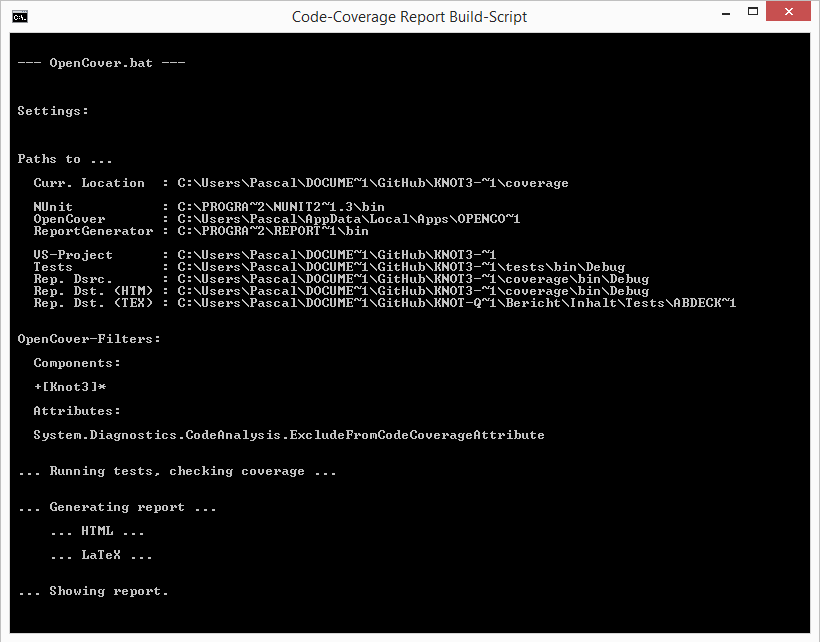
\includegraphics[width=\textwidth]{\Tools/Code-Coverage Report Build-Script.png}
	
	\caption{Build-Batch für die Erstellung des Testabdeckungs-Berichts.}

\end{figure}

~\\
{\hyperref[Abschnitt:Tests:Werkzeuge]{\mousecursor~Zurück zur Beschreibung der Testwerkzeuge auf S. \pageref{Abschnitt:Tests:Werkzeuge}}.}











	
	
	% Verzeichnisse
	%
	% \input{Inhalt/Verzeichnisse/Verzeichnisse}
	
	% Anhänge
	%
	%\input{Inhalt/Anhaenge/Anhaenge}


\end{document}